\section{LTI-Systeme}

Ein LTI-System ist ein System $S$ (Operator), welches eine Funktion $x = x(t)$ auf eine Funktion $y = y(t)$ abbildet und sowohl \textbf{linear}, 
als auch \textbf{zeitinvariant} ist.

\begin{center}
    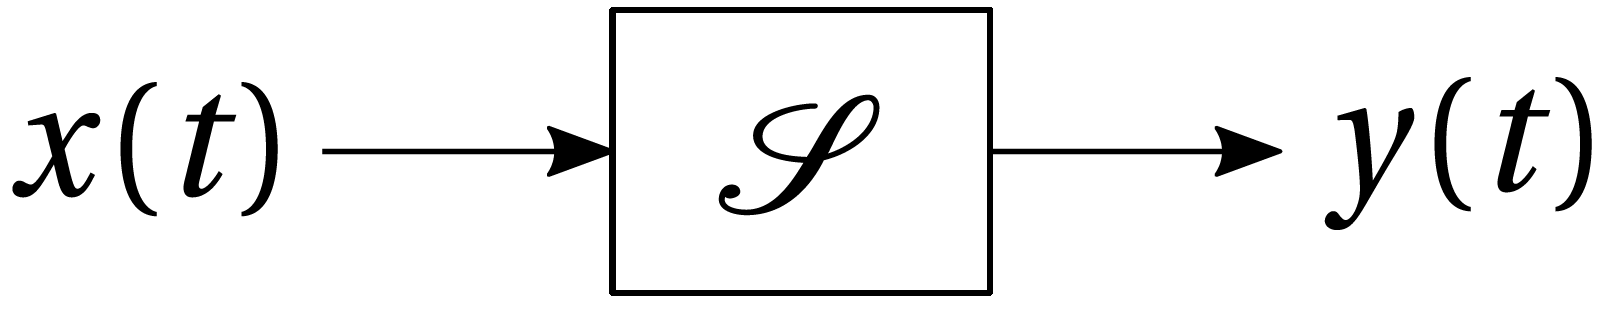
\includegraphics[width=0.7\columnwidth]{images/LTI_system.png}
\end{center}


\begin{tabular}{ll}
    linear          & $S \{ a_1 \cdot x_1(t) + a_2 \cdot x_2(t) \} = a_1 \cdot S \{ x_1(t) \} + a_2 \cdot S \{x_2(t) \}$    \\
                    & für $a,b \in \mathbb{R}$ \qquad (Linearkombination)                                                   \\
    \\
    zeitinvariant   & $S \{ x(t) \} = y(t)$ \textrightarrow\  $S \{ x(t + t_0) \} =  y(t + t_0)$                            \\
                    & für $t_0 \in \mathbb{R}$ \qquad (Zeitverschiebung)                                                    \\
                    & Ein um $t_0$ späteres Eingangssignal bewirkt ein um $t_0$ späteres                                    \\
                    & Ausgangssignal                                                                                        \\
    \\
    Notation        & $S : \, x(t) \mapsto y(t) = S \{x(t) \} = S[x](t)$
\end{tabular}

